
%----------------------------------------------------------------------------------------
%	PART
%----------------------------------------------------------------------------------------


\part{Capítulo siete}
\graphicspath{ {img/ch7/}, {img/} }

%----------------------------------------------------------------------------------------
%	CHAPTER 7
%----------------------------------------------------------------------------------------

\chapterimage{ima2} % Chapter heading image


\chapter{Amortización y Capitalización}
%\begin{center}
%	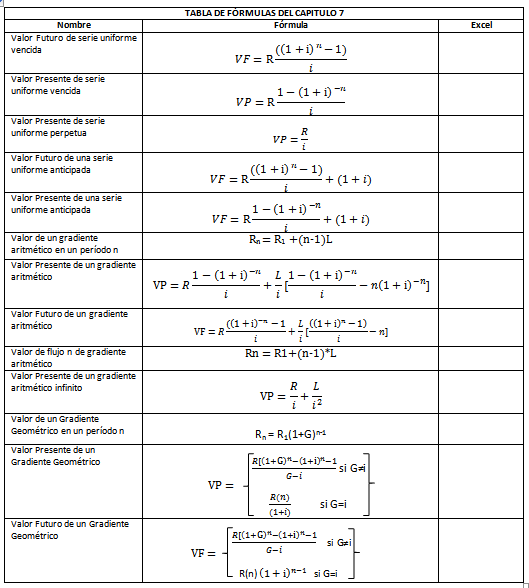
\includegraphics[height=11cm]{7_0}
%\end{center}





\textbf{Ejemplo 1}\\
Se va a cancelar una deuda por \$200.000 en 4 pagos trimestrales de \$R C/U con una tasa de interés de 32\% nominal anual trimestre vencido: 
\\\\
\textbf{a}.	Diagrama de flujo de caja:
\begin{center}
	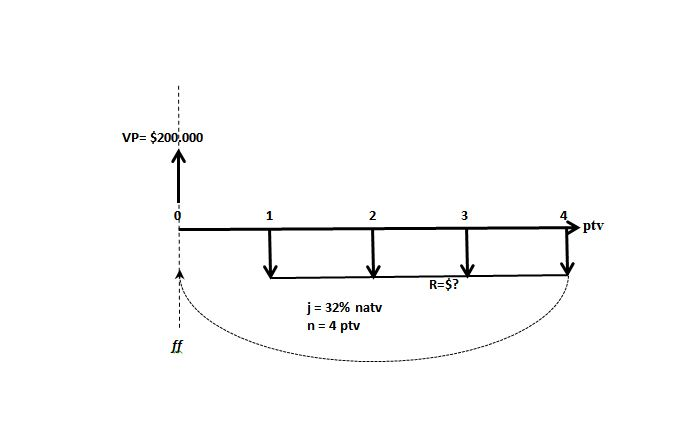
\includegraphics[height=8cm]{7_1}
\end{center}


\textbf{b.} Declaración de variables:\\\\
%\begin{align*}
	%VP=\$ 200.000\\
	j=32\%\ natv\\
	n=4 ptv\\
	R=\$?\\
%\end{align*}

\newpage
\textbf{c.}	Declaración de fórmulas:\\\\
%\begin{align*}
	$VP=R \frac{1-(1+i)^{-n}}{i}$ \hspace{35 pt} \textit{Valor presente serie uniforme vencida}\\
	
	\$200000=R $\frac{1-(1+0,08)^{-4}}{0,08}$\hspace{35 pt} \textit{Ecuación de valor}\\
	
	$R_{n}$ = ?\\
%\end{align*}
\\\textbf{d.} Desarrollo matemático:\\\\
Se despeja R para obtener el resultado de cada una de las cuotas.\\
$R_{1}$ = \$? \\
$R_{2}$ = \$? \\
$R_{3}$ = \$? \\
$R_{4}$ = \$? \\\\
\textbf{e.}Respuesta: \\

	$R=\$ 60.384,16$


Pero si se hace un pago adicional de \$50.000 al final del mes 9, la cuota ordinaria debe bajar porque al plantear la ecuación de valor se debe incluir un pago más y en este caso se dice que esa cuota extra es "pactada" y el diagrama de flujo de caja quedará así:


\textbf{a.} Diagrama de flujo de caja:
\begin{center}
	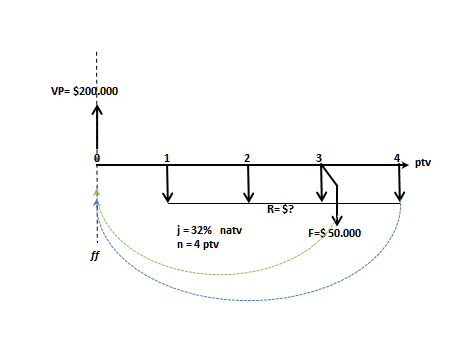
\includegraphics[height=10.5cm]{7_2}
\end{center}
\textbf
\newpage
{b.} Declaración de variables\\\\
%\begin{align*}
    $j=32\% natv \\
	VP=\$ 200.000\\
	n_{1}$=4 \ \ ptv \\
	n_{2}$=3 \ \ ptv  \\
	F=\$50.000\\\\
%\end{align*}
\textbf{c.} Declaración de fórmulas:\\\
%\begin{align*}
    P=F($(1+i)^{-n}$) \hspace{35 pt} \textit{Valor presente dado un valor futuro}\\
	$VP=R\frac{1-(1+i)^{-n}}{i}  \hspace{35 pt} \textit{Valor presente serie uniforme vencida}\\\\
%\end{align*}

\textbf{d.} Desarrollo matemático:\\\\
Se despeja R nuevamente para obtener el resultado de cada una de las cuotas.\\\\
$200.000=R \frac{1-(1+0,08)^{-4}}{0,08}+\$50.000 (1+0,08)^{-3} \hspace{25 pt} \textit{Ecuación de valor}$\\

\textbf{e.} Respuesta:\\
%\begin{align*}
	R=\$ 48.400,44 \\\\
%\end{align*}
Al elaborar la tabla de amortización, se debe tener presente que en el período 3 el valor del pago debe ser igual al pago ordinario más el pago extraordinario, tal como se ve en la siguiente tabla:

\begin{spacing}{1.1}
    \begin{center}
        \begin{tabular}{|p{1cm}|p{2cm}|p{2cm}|p{2cm}|p{3cm}|}
        \hline 
        \rowcolor{white!5}
            \textbf{PER\ (1)} & \textbf{SALDO DEUDA (2)=(2)-(5)} & \textbf{INTERESES  (3)=(2)*(i)}& \textbf{PAGO\ (4)=\$R-\$L }& \textbf{AMORTIZACIÓN  (5)=(4)-(3)} \\ \hline                        

            0 & \$200.000,00 & --------- & --------- & ---------\\ \hline 
            1 & \$167.599,56  &\$ 16.000,00  & \$48.400,44  & \$32.400,44 \\ \hline
            2 & \$132.609,08  &\$ 13.407,96  & \$48.400,44  & \$34.992,48 \\ \hline
            3 & \$44.815,21 & \$10.608,57  & \$98.400,44 & \$87.791,87 \\ \hline
            4 & \$0,00  & \$3.585,23  & \$48.400,44  & \$44.815,21 \\ \hline

 
\end{tabular}
\end{center}
\end{spacing}
\textbf{Ejemplo 2 }\\
Una deuda de \$600.000 se va a cancelar en 7 pagos trimestrales con un interés del 9\% periódico trimestre vencido. Si al momento de efectuar el pago número 3 se efectúa un abono 2 extraordinario, no pactado, de \$250.000. Se pide: a) Elaborar una tabla de amortización sin considerar el abono. b) Elaborar una tabla supoiendo que la cuota extra se abona a capital sin reliquidar la cuota. c) Elaborar una tabla de amortización si al hacer el abono extra se pide reliquidar la cuota.
\\\\
\textbf{a.} Grafica flujo de caja:
\begin{center}
	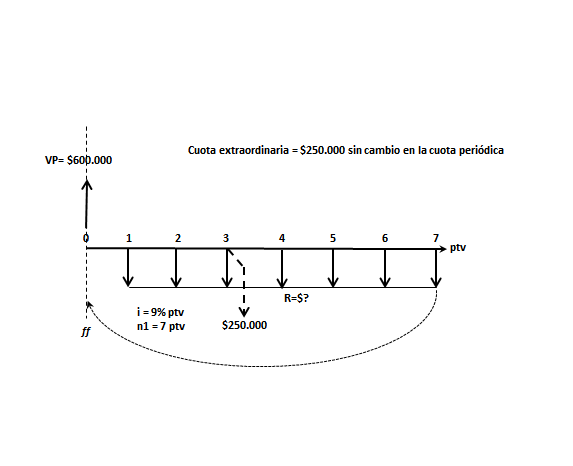
\includegraphics[height=10cm]{7_4}
\end{center}
\textbf{b.} Declaración de variables:\\  
%\begin{align*}
	$VP = $ \$ 600.000\\
	i = 9 \% \ \ ptv\\
	$n_{1}$ = 7\ ptv\\\\
%\end{align*}
\textbf{c.} Declaración de fórmulas:
%\begin{align*}
	$VP=R \frac{1-(1+i)^{-n}}{i} \hspace{35 pt} \textit{Valor presente de una serie uniforme vencida}\\
%\end{align*}
\textbf{d.} Procedimiento:\\

De donde se obtiene R.\\
$\$600.000=R \frac{1-(1+0,09)^{-7}}{0,09}$ \hspace{35 pt} \textit{Ecuación de valor}\\

\textbf{e.} Resultado:
%\begin{align*}
	$R=\$ 119.214,31$\\
%\end{align*}
Ahora elaboramos la tabla sin tener en cuenta ninguna cuota extra puesto que no se han pactado.


\begin{spacing}{1.1}
    \begin{center}
        \begin{tabular}{|p{1cm}|p{2cm}|p{2cm}|p{2cm}|p{3cm}|}
        \hline 
        \rowcolor{white!50}
            \textbf{PER\ (1)} & \textbf{SALDO DEUDA (2)=(2)-(5)} & \textbf{INTERESES  (3)=(2)*(i)}& \textbf{PAGO\ (4)=\$R-\$L }& \textbf{AMORTIZACIÓN  (5)=(4)-(3)} \\ \hline                        

            0 & \$600.000,00 & --------- & --------- & ---------\\ \hline 
            1 & \$534.785,69  &\$ 54.000,00  & \$119.214,31  & \$65.214,31 \\ \hline
            2 & \$463.702,09  &\$ 48.130,71  & \$119.214,31  & \$71.083,60 \\ \hline
            3 & \$386.220,97 & \$41.733,19  & \$119.214,31 & \$77.481,12 \\ \hline
            4 & \$301.766,55  & \$34.759,88  & \$119.214,31  & \$84.454,42 \\ \hline
            5 & \$209.711,23  & \$27.158,99  & \$119.214,31  & \$92.055,32 \\ \hline
            6 & \$109.370,93  & \$18.874,01  & \$119.214,31  & \$100.340,30 \\ \hline
            7 & \$0,00  & \$9.843,38  & \$119.214,31  & \$109.370,93 \\ \hline

 
\end{tabular}
\end{center}
\end{spacing}

La primera forma se puede presentar cuando, al cancelar la tercera cuota, el deudor decide efectuar un abono de \$ 250.000, adicional as u cuota ordinaria periódica, entonces la tabla quedará así:
\begin{spacing}{1.1}
    \begin{center}
        \begin{tabular}{|p{1cm}|p{2cm}|p{2cm}|p{2cm}|p{3cm}|}
        \hline 
        \rowcolor{white!50}
            \textbf{PER\ (1)} & \textbf{SALDO DEUDA (2)=(2)-(5)} & \textbf{INTERESES  (3)=(2)*(i)}& \textbf{PAGO\ (4)=\$R-\$L }& \textbf{AMORTIZACIÓN  (5)=(4)-(3)} \\ \hline                        

            0 & \$600.000,00 & --------- & --------- & ---------\\ \hline 
            1 & \$534.785,69  &\$ 54.000,00  & \$119.214,31  & \$65.214,31 \\ \hline
            2 & \$463.702,09  &\$ 48.130,71  & \$119.214,31  & \$71.083,60 \\ \hline
            3 & \$136.220,97 & \$41.733,19  & \$369.214,31 & \$327.481,12 \\ \hline
            4 & \$29.266,55  & \$12.259,89  & \$119.214,31  & \$106.954,42 \\ \hline
            5 & \$0,00  & \$2.633,99  & \$31.900,54  & \$29.266,55 \\ \hline

 
\end{tabular}
\end{center}
\end{spacing}


El pago del período 5 debe ser igual a los intereses más el saldo de la deuda, esto es:
\begin{align*}
	2.633,99+29.266,55=\$31.900,40
\end{align*}
Obsérvese que la deuda se canceló antes de lo previsto.\\

La segunda forma se puede presentar cuando, al momento de efectuar el pago de la tercera cuota, el deudor desea hacer un abono extra de \$250.000, pero exige reliquidación de la cuota para conservar el plazo originalmente pactado, entonces el capital insoluto o saldo de la deuda del período 3 deberá ser cancelada en los 4 períodos restantes, por tanto la nueva cuota será:\\

\textbf{a.} Diagrama de flujo de caja:
\begin{center}
	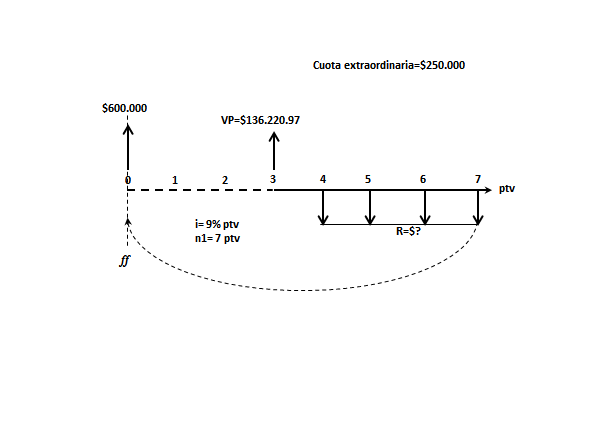
\includegraphics[height=9.5cm]{7_7}
\end{center}
\textbf{b.}	Declaración de variables: \\


	VP=\$ 136.220,97\\
	i=9 \% \ \ ptv\\
	n=4 \ \ ptv\\
	R=\$?\\


\textbf{c.} Declaración de fórmulas:
\begin{align*}
	VP=R \frac{1-(1+i)^{-n}}{i} \hspace{35 pt} \textit{Valor presente serie uniforme}\\
\end{align*}
\textbf{d.} Desarrollo matemático:\\

Después del abono extraordinario de \$250.000 el saldo de la deuda es ahora de \$136.220,97 que se tomará como nuevo capital inicial, por lo tanto:\\
De donde se obtiene R.\\\\
R=\$136.220,97\\\\ $\frac{1-(1+0,09)^{-4}}{0,09}$ \hspace{35 pt} \textit{Ecuación de valor}\\\\
\textbf{e.} Respuesta: \\\

	R=\$ 42.047,14\\

Y la tabla debe ser modificada así:

\begin{spacing}{1.1}
    \begin{center}
        \begin{tabular}{|p{1cm}|p{2cm}|p{2cm}|p{2cm}|p{3cm}|}
        \hline 
        \rowcolor{white!50}
            \textbf{PER\ (1)} & \textbf{SALDO DEUDA (2)=(2)-(5)} & \textbf{INTERESES  (3)=(2)*(i)}& \textbf{PAGO\ (4)=\$R-\$L }& \textbf{AMORTIZACIÓN  (5)=(4)-(3)} \\ \hline                        

            0 & \$600.000,00 & --------- & --------- & ---------\\ \hline 
            1 & \$534.785,69  &\$ 54.000,00  & \$119.214,31  & \$65.214,31 \\ \hline
            2 & \$463.702,09  &\$ 48.130,71  & \$119.214,31  & \$71.083,60 \\ \hline
            3 & \$136.220,97 & \$41.733,19  & \$369.214,31 & \$327.481,12 \\ \hline
            4 & \$106.433,72  & \$12.259,89  & \$42.047,14  & \$29.787,25\\ \hline
            5 & \$73.965,61  & \$9.579,03  & \$42.047,14  & \$32.468,11 \\ \hline
            6 & \$38.575,37  & \$6.656,90  & \$42.047,14  & \$35.390,24 \\ \hline
            7 & \$0,00  & \$3.471,77  & \$42.047,14  & \$38.575,37 \\ \hline

 
\end{tabular}
\end{center}
\end{spacing}


Observe que la cuota ordinaria baja de \$ 119.214,31 a \$ 42.047,14 pero se mantiene el plazo originalmente pactado.\\

\textbf{Ejemplo 3 }\\
Se concede un préstamo de \$2.000.000, con un plazo de gracia muerto de 6 meses seguido de 4 cuotas trimestrales crecientes en un 10\%  y con un interés del 44\% nominal anual trimestre vencido. Elaborar la tabla de amortización.\\

\textbf{Solución:}\\
\textbf{a.} Diagrama de flujo de caja
\begin{center}
	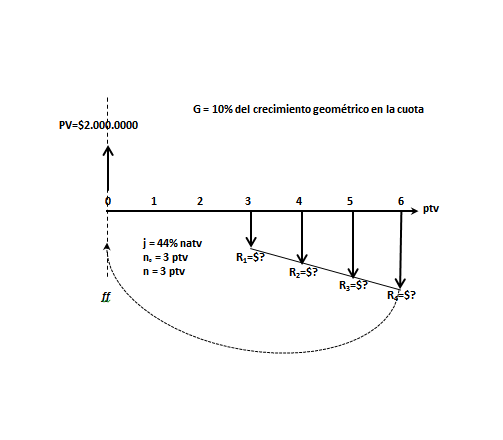
\includegraphics[height=10.50cm]{7_9}
\end{center}
\textbf{b.} Declaración de variables: \\\\

	R_{1}  = \$?\\
	VP=\$2'000.000\\
	G=10 \%  \\
	j=44 \% natv \\
	i=11 \% \ \ ptv\\
	n=4 \ \ ptv\\\\

\textbf{c.} Declaración de fórmulas:\\\\

	$VP=\frac{R[(1+g)^{n}(1+i)^{n}-1]}{(g-i)}$ \hspace{35 pt} \textit{Valor presente gradiente aritmético}\\

\textbf{d.} Desarrollo matemático:\\\\

	$\$ 2.000.000=  \frac{R_{1} [(1+0,1)^{4} (1+0,11)^{-4}-1]}{0,1-0,11}(1+0,11)^{-2}$ \hspace{35 pt} \textit{Ecuación de valor}\\

\textbf{e.} Respuesta:
\begin{spacing}{1.1}
    \begin{center}
        \begin{tabular}{|p{1cm}|p{2cm}|p{2cm}|p{2cm}|p{3cm}|}
        \hline 
        \rowcolor{white!50}
            \textbf{PER\ (1)} & \textbf{SALDO DEUDA (2)=(2)-(5)} & \textbf{INTERESES  (3)=(2)*(i)}& \textbf{PAGO\ (4)=\$R-\$L }& \textbf{AMORTIZACIÓN  (5)=(4)-(3)} \\ \hline                        

            0 & \$2'000.000,00 & --------- & --------- & ---------\\ \hline 
            1 & \$2'000.000,00  &\$ 220.000,00  & \$0,00  & \$-220.000,00 \\ \hline
            2 & \$2'464.200,00  &\$ 244.200,00  & \$0,00  & \$-244.200,00 \\ \hline
            3 & \$2'042.236,06 & \$271.062,00  & \$693.125,94 & \$422.063,94 \\ \hline
            4 & \$1'504.332,50  & \$224.634,97  & \$762.438,53  & \$537.803,56\\ \hline
            5 & \$831.126,69  & \$165.476,58  & \$838.682,39  & \$673.205,81 \\ \hline
            6 & \$0,00  & \$91.423,94  & \$922.550,63  & \$831.126,69 \\ \hline

 
\end{tabular}
\end{center}
\end{spacing}

\textbf{Ejemplo 4}\\
Resolver el problema anterior suponiendo que el plazo de gracia es con cuota reducida al costo de los intereses.\\

\textbf{Solución:}\\
\textbf{a.} Diagrama de flujo de caja:
\begin{center}
	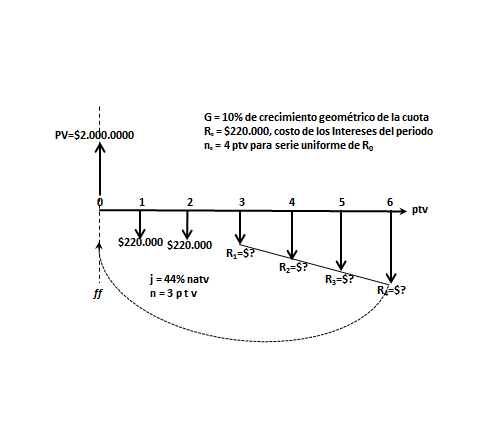
\includegraphics[height=10.50cm]{7_11}
\end{center}
\textbf{b.} Declaración de variables:\\\\

	$R_{1}  = \$?\\
	R_{2}  = \$?\\
	R_{3}  = \$?\\
	R_{4}  = \$?\\
	VP=\$2.000.000 \\
	g=10 \%\ \\
	j=44 \% \ \ natv\\
	i=11 \%\ ptv\ \\
	n=4 \ \ ptv\\
	R_{0}=\$ 220.000$\\

\textbf{c.} Declaración de fórmulas:\\\\

	$VP=\frac{R[(1+G)^{n}(1+i)^{n}-1]}{(G-i)}$ \hspace{35 pt} \textit{Valor presente gradiente geométrico}\\
	
	\\
	$\$ 2.000.000=  \frac{R_{1} [(1+0,1)^{4} (1+0,11)^{-4}-1]}{0,1-0,11}(220.000(i+0,11)^{-2})$ \hspace{35 pt} \textit{Ecuación de valor}
	
	\\\\
	$R =  \frac{(1-(1+0,11)^{-2})}{0,11}$ \\

\textbf{e.} Respuesta\\
$	R_{1}=\$ 562.556,56$

\begin{spacing}{1.1}
    \begin{center}
        \begin{tabular}{|p{1cm}|p{2cm}|p{2cm}|p{2cm}|p{3cm}|}
        \hline 
        \rowcolor{white!50}
            \textbf{PER\ (1)} & \textbf{SALDO DEUDA (2)=(2)-(5)} & \textbf{INTERESES  (3)=(2)*(i)}& \textbf{PAGO\ (4)=\$R-\$L }& \textbf{AMORTIZACIÓN  (5)=(4)-(3)} \\ \hline                        

            0 & \$2'000.000,00 & \$0,00 & \$0,00 & \$0,00 \\ \hline 
            1 & \$2'000.000,00  &\$ 220.000,00  & \$220.000,00  & \$0,00 \\ \hline
            2 & \$2'000.000,00  &\$ 220.200,00  & \$220.000,00  & \$0,00 \\ \hline
            3 & \$1'657.443,44 & \$220.000,00  & \$562.556,56 & \$342.556,56 \\ \hline
            4 & \$1'220.950,00  & \$182.318,78  & \$618.812,22  & \$436.493,44\\ \hline
            5 & \$674.561,06  & \$1134.304,50  & \$680.693,44  & \$546.388,94 \\ \hline
            6 & \$0,00  & \$74.201,72  & \$748.762,78  & \$674.561,06 \\ \hline

 
\end{tabular}
\end{center}
\end{spacing}


\textbf{Ejemplo 5}\\
Elaborar una tabla para amortizar la suma de \$2 millones, en las siguientes condiciones:\\
a)	plazo de gracia muerto 6 meses\\
b)	plazo de gracia con cuota reducida al pago de los intereses \\
c)	4 cuotas uniformes a partir del período 4\\
d)	cuota extraordinaria pactada \$150.000, en el período 7\\
e)	tasa de interés del 21\% nominal anual trimestre vencido\\

\textbf{Solución:}\\
\textbf{a.}	Diagrama de flujo de caja:
\begin{center}
	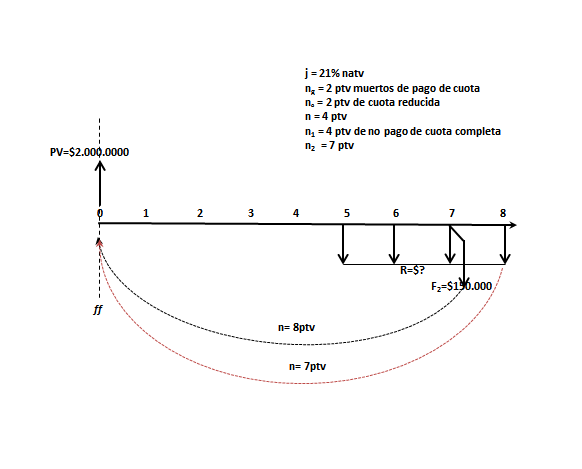
\includegraphics[height=10.00cm]{7_13}
\end{center}
\textbf{b.} Declaración de variables:\\


	R_{1}  = \$?\\
	VP=\$2.000.000\\
	j=21\%  \ \ natv\\
	i=5,25\%\ ptv\\
	n_{g} = 2\ ptv\\
	R_{0} = \$220.000\\
	n_{0} = 2\ ptv \\
	R_{1} = \$?\ \\
	n_{1} = 4\ ptv\\
	F_{2} = \$150.000\ \\
	n_{2} = 7\ ptv\\
	

\textbf{c.}	Declaración de fórmulas:\\


	$VF=VP(1+i)^{n}$ \hspace{35 pt} \textit{Valor futuro}\\
	$VP=R \frac{(1-(1+i)^{-n})}{i}$ \hspace{35 ptv} \textit{Valor presente de una serie uniforme vencida}\\
	

\textbf{d.}	Desarrollo matemático:\\
Los períodos 1 y 2 son de gracia muertos; los períodos 3 y 4 son de gracia con cuota reducida al valor de los intereses sobre a deuda, capitalizados los intereses en el período de gracia; los períodos 5 al 8 son de cuota ordinaria; en el período 2 la deuda será:
\begin{align*}
	F=P(1+i)^{n}\\
	
\end{align*}
\begin{align*}
	F = \$ 2.000.000 (1+0,0525)^{2}=\$ 2.215.512,50
\end{align*}
El valor del interés $I$ de los períodos 3 y 4, se calcula aplicando la tasa a la deuda que hay en el período 2.
\begin{align*}
	(\$ 2.215.512,50) x (0,0525)=\$ 116.314,41
\end{align*}
La ecuación de valor quedará así:\\


	$\$ 2.000.000=\$ 116.314,41  \frac{1-(1+0,0525)^{-2}}{0,0525}(1,0525)^{-2}+R \frac{1-(1+0,0525)^{-4}}{0,0525}(1,0525)^{-4}+\$ 150.000 (1,0525)^{-7}$\\
	

\textbf{e.}	Respuesta\\
Al despejar R se obtiene R=\$ 591 940.10 y la tabla será: 
\begin{spacing}{1.1}
    \begin{center}
        \begin{tabular}{|p{1cm}|p{2cm}|p{2cm}|p{2cm}|p{3cm}|}
        \hline 
        \rowcolor{white!50}
            \textbf{PER\ (1)} & \textbf{SALDO DEUDA (2)=(2)-(5)} & \textbf{INTERESES  (3)=(2)*(i)}& \textbf{PAGO\ (4)=\$R-\$L }& \textbf{AMORTIZACIÓN  (5)=(4)-(3)} \\ \hline                        

            0 & \$2'000.000,00 & --------- & --------- & ---------\\ \hline 
            1 & \$2'105.000,00  &\$ 105.000,00  & \$0,00  & \$-105.000,00 \\ \hline
            2 & \$2'215.512,50  &\$ 110.512,50  & \$0,00  & \$-110.512,50 \\ \hline
            3 & \$2'215.512,50 & \$116.314,41  & \$116.314,41 & \$0,00\\ \hline
            4 & \$2'215.512,50  & \$116.314,41  & \$116.314,41  & \$0,00\\ \hline
            5 & \$1'739.886,81  & \$116.314,41  & \$591.940,10  & \$475.625,59 \\ \hline
            6 & \$1'239.290,77  & \$91.344,06  & \$591.940,10  & \$500.596,04 \\ \hline
            7 & \$562.413,44  & \$65.062,77  & \$741.940,10  & \$676.877,33 \\ \hline
            8 & \$0,00  & \$29.526,66  & \$591.940,10  & \$562.413,44 \\ \hline

 
\end{tabular}
\end{center}
\end{spacing}
\textbf{Observaciones: }
1)	La amortización de los períodos 1 y 2 es negativa; esto significa que hay una desamortización o aumento de deuda.\\ 
2)	La amortización de los períodos 3 y 4 es cero, debido a que se pagan los intereses.\\
3)	 El valor del pago en el período 5 es igual a la suma del pago ordinario, más el pago extraordinario \$591.940,1 O + \$150.000 * \$741.940,1.\\

\textbf{Ejemplo 6 }\\
Hallar la distribución del pago número 125 (valor de los intereses y del capital amortizado), en una amortización de \$2 millones, mediante pagos mensuales durante 20 años, suponiendo una tasa del 30\% nominal anual mes vencido.\\

\textbf{Solución:}\\
\textbf{a.}	Diagrama de flujo de caja:
\begin{center}
	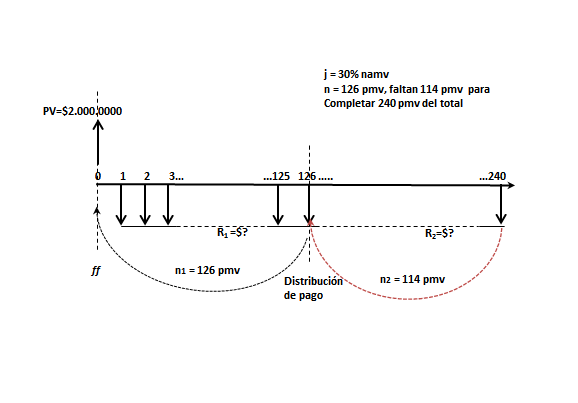
\includegraphics[height=9.50cm]{7_15}
\end{center}
\textbf{b.}	Declaración de variables:\\


	$R = \$?\\
	I=\$?\\
	A=\$?\\
	VP=\$2'000.000\\
	j=30 \% \ \ namv\\
	i=2,5 \% \ \ pmv\\
	n=125\ pmv$\\

\textbf{c.}	Declaración de fórmulas:\\


	$VP=R \frac{1-(1+i)^{-n}}{i}$ \hspace{35 pt} \textit{Valor presente serie uniforme vencido}\\
	$I=P*i$ \hspace{70 pt} \textit{Interés periodico}\\
	$A=R-I$ \hspace{65 pt} \textit{Amortización a capital, una vez descontados os intereses de la cuota R.}\\
	

\textbf{d.}	Desarrollo matemático:\\

Como todos los pagos son iguales, entonces el valor del pago 125 se obtiene de la siguiente ecuación:\\


	$\$2.000.000=R \frac{(1-(1+0,025))^{-240}}{0,025} \hspace{35 pt} \textit{Ecuación de valor}
	\\ \ R=\$50.133,78$\\
	
	

Por otra parte se sabe que la porción de la cuota 125 que se utiliza para pagar intereses es igual a la tasa, multiplicada por la deuda que queda inmediatamente después de haberse efectuado el pago número 124. Entonces, para hallar la deuda, en ese momento, debemos calcular el valor presente de los pagos que faltan por hacer. \\

Como en total hay 240 pagos y se han hecho 124 entonces faltan por hacer 116 pagos. El valor presente de estos pagos en el punto 124 será:
\begin{align*}
	VP = \$50.133,78 \frac{(1-(1+0,025))^{-116}}{0,025}=\$1.891. 004,92=deuda \ \ en\ \ La \ \ cuota \ \ 124
\end{align*}
Y los intereses serán:
\begin{align*}
	I=(\$1.891.004,92) x (0,025)= \$47.275,12
\end{align*}
Finalmente, la amortización será igual a la cuota menos intereses
\begin{align*}
	A=(\$50.133,78)-(47.275,12)=\$2.858,66
\end{align*}
\textbf{e.}	Respuesta:\\
Con la información obtenida anteriormente, si queremos, podemos elaborar la tabla de amortización a partir del período 125.
\begin{spacing}{1.1}
    \begin{center}
        \begin{tabular}{|p{1cm}|p{2cm}|p{2cm}|p{2cm}|p{3cm}|}
        \hline 
        \rowcolor{white!50}
            \textbf{PER\ (1)} & \textbf{SALDO DEUDA (2)=(2)-(5)} & \textbf{INTERESES  (3)=(2)*(i)}& \textbf{PAGO\ (4)=\$R-\$L }& \textbf{AMORTIZACIÓN  (5)=(4)-(3)} \\ \hline                        

            124 & \$1'891.004,92 & \$0,00 & \$0,00 & \$0,00\\ \hline 
            125 & \$1'888.146,26  &\$ 47.275,12  & \$50.133,78  & \$2.858,66 \\ \hline
            
\end{tabular}
\end{center}
\end{spacing}

\textbf{Ejemplo 7}\\
Hallar la distribución del pago 58 en una amortización de \$5 millones en pagos mensuales durante 10 años. Suponga que los pagos son crecientes en un 2\% y que la tasa es del 3\% periódico mes vencido. \\

\textbf{Solución:}
\textbf{a.}	Diagrama de flujo de caja:
\begin{center}
	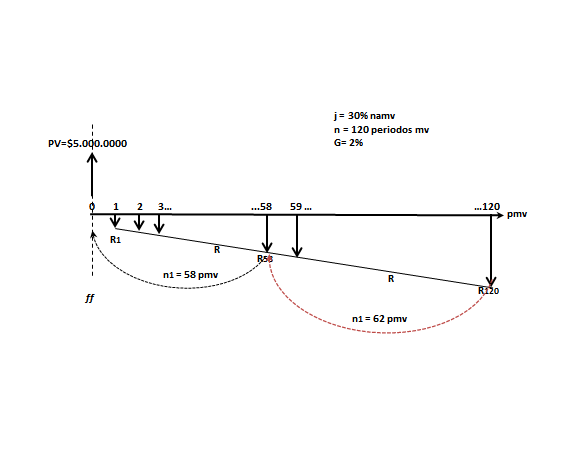
\includegraphics[height=10.00cm]{7_17}
\end{center}
\textbf{b.}	Declaración de variables:\\

%\begin{align*}
	R_{1}  = \$?\\
	VP=\$ 5'000.000\\
	g=2 \%\\
	i=3 \% \ \ pmv\\	
	n=120 pmv\\
	
%\end{align*}
\textbf{c.}	Declaración de fórmulas:\\


	$VP=\frac{R[(1+g)^{n}(1+i)^{n}-1]}{(g-i)} \hspace{35 pt} \textit{Valor presente de un gradiente geométrico si $g\not=$ i}\\
	I = P*i \hspace{95 pt} \textit{Intereses periódicos}\\
	A = R-I \hspace{95 pt} \textit{Amortización a capital, una vez descontados los intereses de la cuota R}\\
	R_{n} = R_{1}(1+g)$\\
	

\textbf{d.}	Desarrollo matemático:\\
Primero debemos calcular $R_{1}$ con el fin de poder hallar el valor de $R_{58}$ y saber qué es lo que va a repartir.\\


	$\$ 5'000.000=\frac{R_{1} [(1,02)^{120}(1,03)^{-120}-1]}{(0,02-0,03)} \hspace{35 pt} \textit{Ecuación de valor}$ \ \ \\
	
	$R_{1}=\$ 72.478,16$ \\


\textbf{e.}	Respuesta\\
Para conocer el valor de $R_{58}$ se aplica la fórmula del último término de un gradiente geométrico.\\

	R_{n}=R_{1}  (1+G)^{n-1} \ \     \\  R_{58}=\$72.478,16 (1+0,02)^{57}=\$224.087,15\\

Para saber qué tanto del pago 58 se destina a intereses, es necesario conocer la deuda en el punto 57 y este valor se multiplica por la tasa de interés.\\

Entonces la deuda en el punto 57 será igual al valor presente en ese punto de lo que falta por pagar, pero lo que falta por pagar es un gradiente geométrico de 63 períodos (120 - 57 = 63) cuyo primer pago es de \$224.087,15, por lo tanto, la deuda en el período 57 será:\\

\textbf{a.}	Diagrama de flujo de caja:\\
\begin{center}
	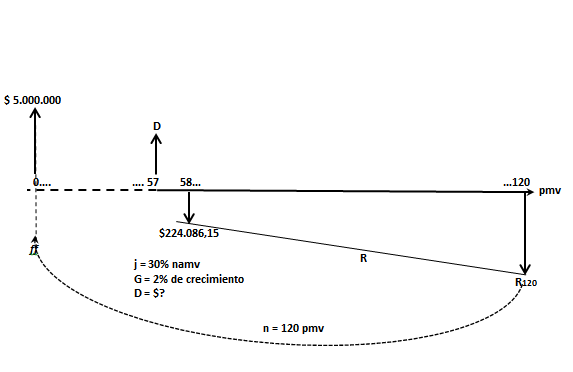
\includegraphics[height=7.00cm]{7_18}
\end{center}
\textbf{b.}	Declaración de variables: \\


	$R_{1}  = \$?\\
	g=2 \%\ \\
	i=3 \% \ \ pmv\\
	D=?\\
	n=63 p(días)vencido\$\\

\textbf{c.}	Declaración de fórmulas:\\


	$VP=\frac{R[(1+g)^{n}(1+i)^{n}-1]}{(g-i)} \hspace{35 pt} \textit{Valor presente de un gradiente geométrico si g $\not=$ i}$\\


\textbf{d.}	Desarrollo matemático:\\


	$VP=\frac{\$224. 087,15[(1,02)^{63}(1,03)^{-63}-1]}{(0,02-0,03)}\\
	
	VP=\$ 10'289.273,19$\\

\textbf{e.}	Respuesta:\\
Los intereses para el período 58 serán:$ \$ 10'289.273,19 x 0,03=\$308.678,20$\\
Amortización = pago - interés = $\$224.087,15 - 308. 678,20= - \$84.591,05$\\

\textbf{Ejemplo 8 }\\
Una persona solicita a una entidad bancaria un préstamo por \$500.000. Lo cancelará en pagos trimestrales, durante un año, con amortización constante a capital e intereses del 33\% nominal anual trimestres anticipado. Elaborar una tabla de amortización.\\

\textbf{ Solución:}\\
\textbf{a.}	Diagrama de flujo de caja:
\begin{center}
	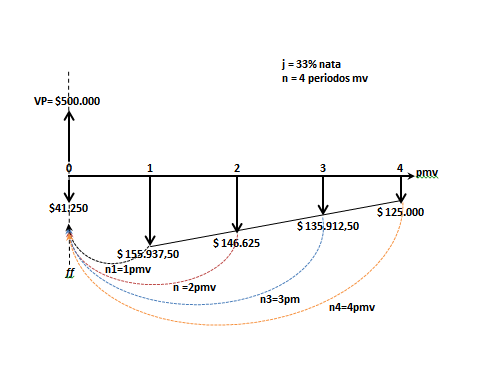
\includegraphics[height=9.50cm]{7_19}
\end{center}
\textbf{b.}	Declaración de variables:\\


	$j_{a}=33\% \ \ nata\\
	i_{a}=\frac{33\% \ \ nata}{4\ pta}=8,25\%\ pta\\
	n=4 \ \ pta\\
	VP=\$ 500.000\\
	A=Constante\\
	R_{1}=\$?\\
	R_{2}=\$?\\
	R_{3}=\$?\\
	R_{4}=\$?$\\


\textbf{c.}	Declaración de fórmulas:\\


	$A=\frac{VP}{n} \hspace{35 pt} \textit{Amortizaión de capital iguales en n períodos, variará el monto de los intereses}\\
	I = P*i \hspace{35 pt} \textit{monto de intereses periódicos}\\
	R = A + i$\\


\textbf{d.}	Desarrollo matemático:\\


La deuda debe ser cancelada con 4 pagos trimestrales, por lo tanto la amortización será:\\


$	A = \frac{\$ 500.000}{4}\ pta$\\

	$\frac{\$ 500.000}{4}=\$ 125.000$\\
	

Al comienzo de la deuda, es decir en el período cero, se cobran intereses de:\\


$	I = \$ 500.000 x 0,0825=\$ 41.250$

Puesto que en el período cero no hay abono a capital, la cuota será igual a los intereses es decir a \$41.250. En el punto 1 de la línea de tiempo, esto es, al final del primer trimestre, debe hacerse un abono a capital de \$125.000, quedando una deuda de \$375.000 y, habrá que pagar los intereses por anticipado sobre \$375.000, entonces, el pago total deberá ser de:
\begin{align*}
	R_{1}=\$125.000 +\$375.000 x 0,0825= \$155. 937,50
\end{align*}
\textbf{e.}	Respuesta:\\
La gráfica y la correspondiente tabla se muestran a continuación.
\begin{center}
	\includegraphics[height=3.5cm]{7_20}
\end{center}

\begin{spacing}{1.1}
    \begin{center}
        \begin{tabular}{|p{1cm}|p{2cm}|p{2cm}|p{2cm}|p{3cm}|}
        \hline 
        \rowcolor{white!50}
            \textbf{PER\ (1)} & \textbf{SALDO DEUDA (2)=(2)-(5)} & \textbf{INTERESES  (3)=(2)*(i)}& \textbf{PAGO\ (4)=\$R-\$L }& \textbf{AMORTIZACIÓN  (5)=(4)-(3)} \\ \hline                        

            0 & \$500.000,00 & \$41.250,00 & \$41.250,00 & \$0,00 \\ \hline 
            1 & \$375.000,00  &\$ 30.937,50  & \$155.937,50  & \$125.000,00 \\ \hline
            2 & \$250.000,00  &\$ 20.625,00  & \$145.625,00  & \$125.000,00 \\ \hline
            3 & \$125.000,00 & \$10.312,50  & \$135.312,50 & \$125.000,00 \\ \hline
            4 & \$0,00  & \$0,00  & \$125.000,00  & \$125.000,00\\ \hline
          

 
\end{tabular}
\end{center}
\end{spacing}



\textbf{Ejemplo 9}\\
Hallar el valor de la cuota total que debe ser pagada al final del mes 12, para amortizar una deuda de \$3 millones con pago anticipado de interés y abonos mensuales constantes a capital, durante 4 años, con un interés del 2\% período mes anticipado.\\

\textbf{Solución: }\\
\textbf{a.}	Diagrama de flujo de caja
\begin{center}
	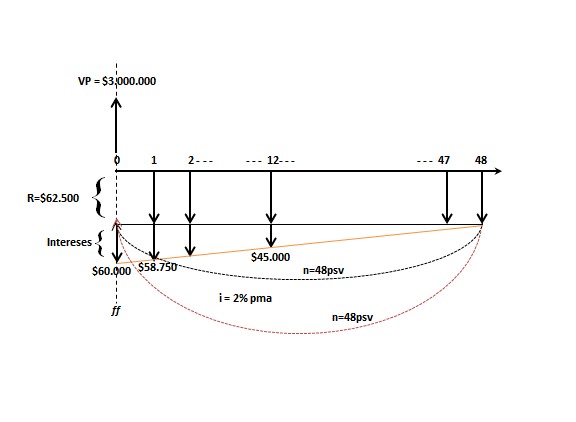
\includegraphics[height=10.00cm]{7_22}
\end{center}
\textbf{b.}	Declaración de variables:\\


	$I=F*i_{a} \hspace{35 pt} \textit{Monto de intereses periódicos anticipados}\\
	A=\frac{P}{n} \hspace{35 pt} \textit{Amortización igual a capital en n períodos}\\
	R=A+i$ \\


\textbf{c.}	Declaración de fórmulas:
\begin{align*}
	VP=\frac{R}{i}
\end{align*}
\textbf{d.} Desarrollo matemático:
Se puede observar que entre el primer pago de intereses que se hace en el período cero (por ser anticipado) y el último pago de intereses (período 47) forma un gradiente lineal decreciente, mientras que el primer abono a capital se hace en el período 1 (por ser vencido).\\

Como los intereses forman un gradiente lineal decreciente, necesitamos calcular el valor L de decrecimiento en la siguiente forma:\\

Interés del período cero: 
\begin{align*}
	I=\$ 3.000.000x0,02= \$60,000
\end{align*}
Deuda al final del primer período:
\begin{align*}
	I=\$ 3.000 000-\$ 62.500= \$ 2.937.500
\end{align*}
Interés al final del primer período: 
\begin{align*}
	I=\$ 2.937.500* 0,02= \$58.750
\end{align*}
Variación del interés:
\begin{align*}
	L= \$1.250
\end{align*}
Ahora, necesitamos calcular los intereses al final del período 12 que corresponden al pago número 13 del gradiente:\\

\
	$R_{13}=R_{1}  + (n-1)L=\$60.000 + (13 -1)( -\$1. 250)= \$45.000$\\
	

El pago que debe hacerse al final del período 12 será igual a la suma de la cuota de interés, más la cuota de abono a capital, esto es:\\


    $R_{13}=\$ 45.000 +\$ 62.500= \$107.500$\\
    

Otra forma de resolver el problema anterior es calculando la deuda en el punto 12 y multiplicando por la tasa.\\

\textbf{e.}	Respuesta:\\

Como en total hay 48 pagos y ya se han hecho 12, faltan 36 pagos por hacer, esto es:\\


    F=36 pma x \$62.500=\$225.000\\
	36 x \$ 62.500= \$2.250.000 \\
	

Intereses:


	F=\$ 2'250.000 x 0,02= \$45.000\\


Valor total de la cuota:\\

    R=A+I\\


	R=\$ 62.500 +\$ 45.000= \$107.500\\


\textbf{Ejemplo 10 }\\
Elaborar una tabla para amortizar la suma de \$300. 000, con un interés del 32\% nominal anual semestre vencido, mediante pagos semestrales, durante 3 años, bajo las siguientes condiciones:\\

a)	la cuota anual aumenta en \$60.000 \\
b)	la intercuota aumenta en \$25.000 cada año \\
c)	la intercuota aumenta un 25\% cada año\\

\textbf{Solución a:}\\
\textbf{a.}	Diagrama de flujo de caja:\\
Primero construimos una gráfica que muestre la forma como va a ser pagada la deuda (esto corresponde a la gráfica del gradiente escalonado), en seguida, construimos la gráfica que muestra los pagos anuales crecientes linealmente en \$60.000 (que corresponde al gradiente lineal simple)
\begin{center}
	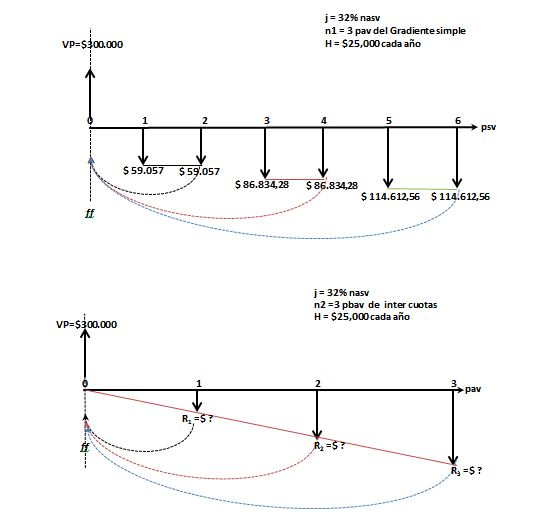
\includegraphics[height=10.5cm]{7_23}
\end{center}
\textbf{b.}	Declaración de variables:\\
Gradiente escalonado:\\


	m=2 \ \ psv\\
	i=16 \% \ \ psv\\
	j=32 \% \ \ nasv\\
	

Gradiente lineal simple:\\


	L=\$ 60.000\\
	n=3 \ \ pav\\
	i= ?\%\\
	

\textbf{c.}	Declaración de fórmulas:\\


	$(1+i_{1})^{m_{1}}=(1+i_{2})^{m_{2}} \hspace{35 pt} \textit{Equivalente de tasas periódicas vencidas}\\
	VP=R \frac{1-(1+i)^{-n}}{i} \hspace{35 pt} \textit{Valor presente gradiente aritmético}\\
	VF=R \frac{((1+i)^{n}-1)}{i} \hspace{35 pt} \textit{Valor futuro de serie uniforme vencida}\\
	R_{n}=R_{1}+(n-1)L\hspace{35 pt} \textit{Valor de un gradiente aritmético en un período n}$\\


\textbf{d.}	Desarrollo matemático:\\
Como los períodos del gradiente son anuales, debemos buscar una tasa nominal equivalente anual al 16\% periódico semestral.\\

Entonces:\\


	$(1 + 0.16)^{2}  = (1 + i)^{1} \\   i = 34.56\%\ pav$\\

Ahora planteamos la ecuación de valor del gradiente simple.
\begin{align*}
	\$300 000= R_{1}x\frac{1-(1+0,3456 \%)^{3}}{(0,3456 \%)}+\frac{60 000}{0.3456}x[\frac{1-(1+0,3456 \%)^{3}}{0,3456 \%}-3 (1+0.3456)^{-3}]
\end{align*}
De donde se obtiene que, \\


	R_{1}  = \$127 563.13\\
	R_{2}= \$187 563.13\ \ y\ \ R_{3}  =\$247.563,13\\

Ahora pasamos a trabajar con el gradiente escalonado, teniendo en cuenta que cada cuota de gradiente debe ser reemplazada por dos intercuotas.\\

\textbf{e.}	Respuesta:\\
El valor final de las intercuotas $r_{1}$ y $r_{2}$ debe ser equivalente a $R_{1}$; el valor final de las intercuotas se calcula con la tasa del 16\% periódica semestral vencido, debido a que las intercuotas son semestrales y partiendo del supuesto que $r_{1}  = r_{2}$  se tiene: \\


$	R_{1}=R_{2}  \frac{((1+16\%)^{2}-1)}{0,16} \ \ \rightarrow \ \ R_{1}=R_{2}  \frac{\$127.563,13}{2,16}=\$59.057\\
	R_{2}=R_{3}  \frac{((1+16\%)^{2}-1)}{0,16} \ \ \rightarrow \ \ R_{3}=R_{4}  \frac{\$187.563, 13}{2,16}=\$86.834,78\\
	R_{3}=R_{5}  \frac{(1+16\%)^{2}-1}{0,16} \ \ \rightarrow \ \ R_{2}=R_{6}  \frac{\$247.563,13}{2,16}=\$114.612,56$\\
	

Ahora, procedemos a elaborar la tabla de amortización usando las intercuotas y una tasa del 16\% periódica semestral vencida.

\begin{spacing}{1.1}
    \begin{center}
        \begin{tabular}{|p{1cm}|p{2cm}|p{2cm}|p{2cm}|p{3cm}|}
        \hline 
        \rowcolor{white!50}
            \textbf{PER\ (1)} & \textbf{SALDO DEUDA (2)=(2)-(5)} & \textbf{INTERESES  (3)=(2)*(i)}& \textbf{PAGO\ (4)=\$R-\$L }& \textbf{AMORTIZACIÓN  (5)=(4)-(3)} \\ \hline                        

            0 & \$300.000,00 & \$0,00 & \$0,00 & \$0,00 \\ \hline 
            1 & \$288.943,00  &\$ 48.000,00  & \$59.057,00  & \$11.057,00 \\ \hline
            2 & \$276.116,88  &\$ 46.230,88  & \$59.057,00  & \$12.826,12 \\ \hline
            3 & \$233.460,80 & \$44.178,70  & \$86.834,78 & \$42.656,08 \\ \hline
            4 & \$183.979,75  & \$37.353,73  & \$86.834,78  & \$49.481,05\\ \hline
            5 & \$98.803,95  & \$29.436,76  & \$114.612,56  & \$85.175,80 \\ \hline
            6 & \$0,00  & \$15.808,61  & \$114.612,56  & \$98.803,95 \\ \hline

 
\end{tabular}
\end{center}
\end{spacing}


\textbf{Solución b:}\\
\textbf{a.}	Diagrama de flujo de caja:\\
Con altura del escalón de \$25 000.
\begin{center}
	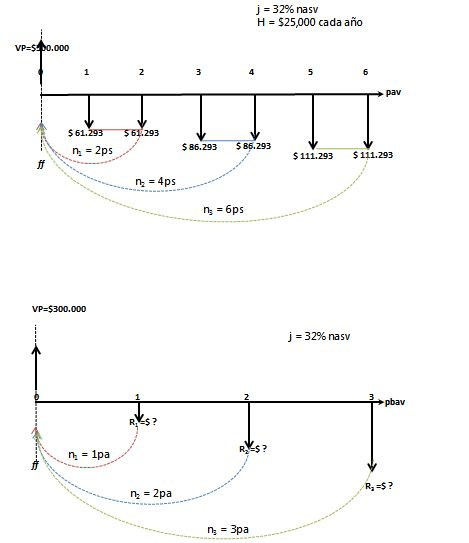
\includegraphics[height=10.5cm]{7_25}
\end{center}
Observase que la diferencia entre estas dos gráficas y las dos anteriores está, en qué y en  las dos primeras, se conocía L = \$ 60.000 y en las dos gráficas de arriba L es desconocido pero sabemos que H = \$ 25 000.\\

\textbf{b.}	Declaración de variables:\\
Gradiente escalonado:\\


	H =\$ 25.000\\
	m=2\ \ psv\\
	i=16\% \ \ psv\\

Gradiente lineal simple:\\


	L=\$ 60.000\\
	n=3 pav\\
	i= 34.56 \%\ \ pav

\textbf{c.}	Declaración de fórmulas:\\


	$VP=R \frac{1-(1+i)^{-n}}{i} \hspace{35 pt} \textit{Valor presente de serie uniforme vencida}\\
	VF=R \frac{(1+i)^{n}-1}{i} \hspace{35 pt} \textit{Valor futuro de serie uniforme vencida}$\\


\textbf{d.}	Desarrollo matemático:\\
Lo primero que debemos hacer es calcular el valor de $L$ , puesto que el dato que tenemos es la altura del escalón. Si la altura del escalón $H$ es \$25.000 corresponderá a la diferencia entre $r_{3}-r_{2}$, o también  $r_{5}-r_{4}$ Entonces:
\begin{align*}
	L = R_{2}  -R_{1} \hspace{35 pt} \textit{Valor del gradiente aritmético}\\
\end{align*}
Ecuación de valor:\\
\begin{align*}

	R_{3}\frac{(1+16\%)^{2}-1}{16\%}-R_{2}\frac{(1+16\%)^{2}-1}{16\%}=(R_{3}-R_{2})\frac{(1+16\%)^{2}-1}{16\%}=H \frac{(1+16\%)^{2}-1}{16\%} \\ %\hspace{35 pt} \textit{Ecuación de valor}\\
\end{align*}
Donde se concluye que:
\begin{align*}
	L=\$ 25.000 \frac{(1+16\%)^{2}-1}{16\%}=\$ 54.000
\end{align*}
Si lo reemplazamos en la formula tenemos: \\


	$\$ 300.000=R_{1} \frac{1-(1+0,3456)^{-3}}{ 0.3456}+\frac{\$54 000}{0.3456}x[\frac{1-(1+0,3456)^{-3}}{0.3456}-3 (1+0,3456)^{-3}] \hspace{35 pt} \textit{Ecuación de valor}$\\


De donde se obtiene $R_{1}= \$ 132 392.88$, y
\begin{align*}
	R_{1}=\$ 132.392,88 \frac{(1+16\%)^{2}-1}{16\%}\ \ \rightarrow\ \ r_{1}=r_{2}  = \$ 61.293,00
\end{align*}
\textbf{e.}	Respuesta:\\
En igual forma se pueden calcular las otras intercuotas, sin embargo, como sabemos que crecerán en forma escalonada en \$25 000 puede usarse este otro procedimiento:\\

	$R_{3}=R_{4}= \$61.293,00+\$25.000,00 = \$86.293,00\\
	R_{5}=R_{6}= \$86.293,00+\$25.000,00 = \$111.293,00$\\


\begin{spacing}{1.1}
    \begin{center}
        \begin{tabular}{|p{1cm}|p{2cm}|p{2cm}|p{2cm}|p{3cm}|}
        \hline 
        \rowcolor{white!50}
            \textbf{PER\ (1)} & \textbf{SALDO DEUDA (2)=(2)-(5)} & \textbf{INTERESES  (3)=(2)*(i)}& \textbf{PAGO\ (4)=\$R-\$L }& \textbf{AMORTIZACIÓN  (5)=(4)-(3)} \\ \hline                        

            0 & \$300.000,00 & \$0,00 & \$0,00 & \$0,00 \\ \hline 
            1 & \$286.707,00  &\$ 48.000,00  & \$61.293,00  & \$13.293,00 \\ \hline
            2 & \$271.287,12  &\$ 45.873,12  & \$61.293,00  & \$15.419,00 \\ \hline
            3 & \$228.400,06 & \$43.405,95  & \$86.293,00 & \$42.887,06 \\ \hline
            4 & \$178.651,075  & \$36.544,01  & \$86.293,00  & \$49.748,99\\ \hline
            5 & \$95.942,24  & \$28.584.17  & \$111.293,00  & \$82.708,83 \\ \hline
            6 & \$0,00  & \$15.350,76  & \$111.293,00  & \$95.942,24 \\ \hline

 
\end{tabular}
\end{center}
\end{spacing}


\textbf{Solución c:}\\
\textbf{a.}	Diagrama de flujo de caja:
\begin{center}
	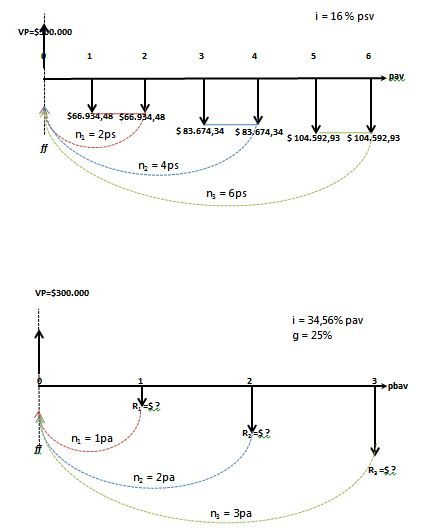
\includegraphics[height=10.0cm]{7_27}
\end{center}
\textbf{b.}	Declaración de variables:\\
Gradiente escalonado:\\
	
	i=16\% \ \ psv \\
	m=2  psv\\

Gradiente geométrico:\\

	g=25 \%\\
	i= 34,56 \% pav \\
	n=3\ \ pav\\
	

\textbf{c.}	Declaración de fórmulas:
\begin{align*}
	VP=\frac{R[(1+G)^{n}(1+i)^{n}-1]}{(G-i)} \hspace{35 pt} \textit{Valor presente gradiente geométrico}\\
\end{align*}
\textbf{d.}	Desarrollo matemático:\\
Procedemos en forma similar como lo hicimos en el caso a), pero usaremos la fórmula del gradiente geométrico.\\

Entonces:
\begin{align*}
	\$ 300.000=\frac{R_{1} [(1+0,25)^{3} (1+0,3456)^{-3}-1]}{0,25-0,3456} \hspace{35 pt} \textit{Ecuación de valor}\\
\end{align*}
 $R_{1}  = \$225.920,73$\\

\textbf{e.}	Respuesta:\\
El cálculo de las intercuotas se hace en forma similar, al realizado en el literal a)\\


	$R_{1}=R_{2}=\$66.939,48 \\
	R_{3}=R_{4}= \$83.674,34 \\
	R_{5}=R_{6}= \$ 104.592,93$\\



\begin{spacing}{1.1}
    \begin{center}
        \begin{tabular}{|p{1cm}|p{2cm}|p{2cm}|p{2cm}|p{3cm}|}
        \hline 
        \rowcolor{white!50}
            \textbf{PER\ (1)} & \textbf{SALDO DEUDA (2)=(2)-(5)} & \textbf{INTERESES  (3)=(2)*(i)}& \textbf{PAGO\ (4)=\$R-\$L }& \textbf{AMORTIZACIÓN  (5)=(4)-(3)} \\ \hline                        

            0 & \$300.000,00 & \$0,00 & \$0,00 & \$0,00 \\ \hline 
            1 & \$281.060,52  &\$ 48.000,00  & \$66.939,48  & \$18.939,48 \\ \hline
            2 & \$259.090,72  &\$ 44.969,68  & \$66.939,48  & \$21.969,80 \\ \hline
            3 & \$216.870,9006 & \$41.454,52  & \$83.674,34 & \$42.219,82 \\ \hline
            4 & \$167.895,90  & \$34.699,34  & \$83.674,34  & \$48.975,00\\ \hline
            5 & \$90.166,31  & \$26.863,34  & \$104.592,93  & \$77.729,59 \\ \hline
            6 & \$0,00  & \$14.426,62  & \$104.592,93  & \$90.166,31 \\ \hline

 
\end{tabular}
\end{center}
\end{spacing}



\textbf{Ejemplo 11}\\
Elaborar una tabla para amortizar la suma de \$600.000 en 4 pagos anuales e iguales, pero en valor constante, suponga una tasa de interés del 8\% periodo trimestre vencido y que:\\

a)	la corrección monetaria permanecerá constante en el 22\% durante los 4 años.\\
b)	la corrección monetaria es del 22\% en los 2 primeros años, del 24\% para el tercer año y del 27\% para el cuarto año.\\

\textbf{Solución a:}\\
\textbf{a.}	Diagrama de flujo de caja:
\begin{center}
	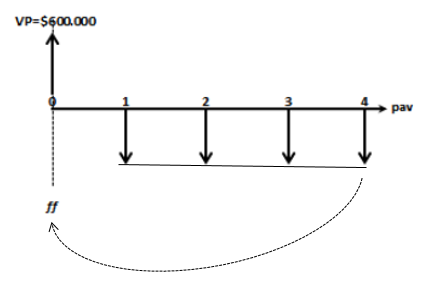
\includegraphics[height=5.0cm]{7_29}
\end{center}

\textbf{b.}	Declaración de variables:\\

    VP=\$ 600.000\\
	i=8 \% \ \ ptv\\
	n=4 \ \ pav\\
	R= \$?\\

\textbf{c.}	Declaración de fórmulas:\\

	$VP=R \frac{1-(1+i)^{-n}}{i} \hspace{35pt}\textit{Valor presente serie uniforme vencida}$\\

\textbf{d.}	Desarrollo matemático:\\
Primero calculamos el valor de la cuota haciendo caso omiso de la corrección monetaria\\


	$\$ 600.000= R \frac{1-(1+0,08)^{-4}}{0,08}$ \\
	
	R=\$ 181.152,48\\
	
El valor de \$181.152,48 corresponde al valor de las cuotas pero en pesos de hoy, sin embargo, cuando se vaya a pagar la primera cuota este valor se debe incrementar debido a la corrección monetaria y será:\\

Primera cuota:	 $\$181.152,48 x (1 +0,22)   =\$221.006,03$\\
Segunda cuota:	 $\$181.152,48 x (1 +0.22)^{2}=\$269 627.35$\\
Tercera cuota:	 $\$181.152,48 x (1 +0.22)^{3}=\$328.945,37$ \\
Cuarta cuota:	 $\$181.152,48 x (1 +0,22)^{4}=\$401.313,35$ \\

Así como hemos corregido el valor de las cuotas tenemos que corregir los saldos de la deuda y para ello será necesario incluir en la tabla una nueva columna que denominaremos ''capital insoluto ajustado'', donde colocaremos, los saldos de la deuda ajustados con la corrección monetaria al final de cada período.\\

\textbf{e.	}Respuesta:\\
El saldo insoluto ajustado del período cero se obtiene al aplicarle la corrección monetaria al saldo insoluto del período cero, esto es:
\begin{align*}
	\$600.000 x (1+0,22)=\$732.000
\end{align*}
Sobre los \$732.000 se calculan los intereses así:
\begin{align*}
	\$732.000 x 0,08=\$58.560,00 
\end{align*}
Si al saldo ajustado del período cero se le resta la amortización se tendrá el saldo (sin ajustar) al comienzo del primer período así:
\begin{align*}
	\$732.000-\$162.446,03=\$569.553,97 
\end{align*}
Este saldo se deberá ajustar para saber cuál es la deuda al final del mismo período, entonces se tendrá:
\begin{align*}
	\$569.553,97 x (1 +0,22)=\$694.855,84 
\end{align*}
Al saldo insoluto ajustado del período 1 se le aplica la tasa de interés para obtener los intereses así:
\begin{align*}
	\$694.855,84 x 0,08 =\$55.588,47
\end{align*}
El resto de la tabla continúa en forma similar:

\begin{spacing}{1.1}
    \begin{center}
        \begin{tabular}{|p{1cm}|p{3cm}|p{2cm}|p{2cm}|p{2cm}||p{3cm}|}
        \hline 
        \rowcolor{white!50}
            \textbf{PER\ (1)} & \textbf{SALDO AJUSTADO } & \textbf{SALDO (3)=(3)-(6)} & \textbf{INTERESES  (4)=(3)*(i)}& \textbf{PAGO\ (5)=\$R-\$L }& \textbf{AMORTIZACIÓN  (6)=(5)-(4)} \\ \hline                        

            0 & \$600.000,00 & \$732.000,00 & \$0,00 & \$0,00 & \$ 0,00\\ \hline 
            1 & \$569.553,97  &\$ 694.855,84  & \$58.560,00  & \$221.006,03 & \$ 214.038,88 \\ \hline
            2 & \$480.816,96  &\$ 371.586,45  & \$46.927,74  & \$328.945,37 &\$282.017,64 \\ \hline
            3 & \$304.779,06 & \$371.586,45  & \$46.927,74 & \$328.945,37 & \$282.017,64 \\ \hline
            4 & \$0,00  & \$0,00  & \$29.726,90  & \$401.313,35 & \$371.586,45\\ \hline
          

 
\end{tabular}
\end{center}
\end{spacing}


\textbf{Solución b:}\\
Igual que en la parte a) calculamos el valor de la cuota haciendo caso omiso de la corrección monetaria y el valor de ésta, resulta ser en pesos de hoy, \$181 152.48, y el valor de lo que se debe pagar anualmente, será:\\

Primera cuota:	 $\$181.152,48 x (1 +0,22)   =\$221.006,03$\\
Segunda cuota:	 $\$181.152,48 x (1 +0,22)^{2}=\$269.627,35$\\
Tercera cuota:	 $\$181.152,48 x (1 +0,22)^{2}  x (1 +0,24)=\$334.337,91 $\\
Cuarta cuota:	 $\$181.152,48 x (1 +0,22)^{2}  x (1+0,24)X (1+0,27)=\$424.609,15$\\

Al elaborar la tabla debe tenerse en cuenta que el factor de ajuste del capital insoluto del período 2 será: (1 +0,24) y el factor de ajuste del capital insoluto del período 3 será (1 +0,27) y la tabla quedará así:

\begin{spacing}{1.1}
    \begin{center}
        \begin{tabular}{|p{1cm}|p{2cm}|p{3cm}|p{2cm}|p{2cm}||p{3cm}|}
        \hline 
        \rowcolor{white!50}
 \textbf{PER\ (1)}  & \textbf{SALDO (2)=(2)-(6)}& \textbf{SALDO AJUSTADO } & \textbf{INTERESES  (4)=(2)*(i)}& \textbf{PAGO\ (5)=\$R-\$L }& \textbf{AMORTIZACIÓN  (2)=(5)-(4)} \\ \hline                                    

            0 & \$600.000,00 & \$732.000,00 & \$0,00 & \$0,00 & \$ 0,00\\ \hline 
            1 & \$569.553,97  &\$ 694.855,84  & \$58.560,00  & \$221.006,03 & \$ 162.446,03 \\ \hline
            2 & \$480.816,96  &\$ 596.213,03  & \$55.588,47  & \$269.627,35 &\$214.038,88 \\ \hline
            3 & \$309.572,16 & \$393.156,64  & \$47.697,04 & \$334.337,91 & \$286.640,87 \\ \hline
            4 & \$0,00  & \$0,00  & \$31.452,51  & \$424.609,51 & \$424.609,15\\ \hline
          

 
\end{tabular}
\end{center}
\end{spacing}


\textbf{Ejemplo 12}\\
Amortizar en valor constante la suma de \$500.000 mediante 3 pagos anuales que decrecen en \$20.000; suponga un interés del 10\% periódico anual vencido  y una tasa única de corrección monetaria del 24\% efectivo anual.\\

\textbf{Solución:}\\
\textbf{a.}	Diagrama de flujo de caja:
\begin{center}
	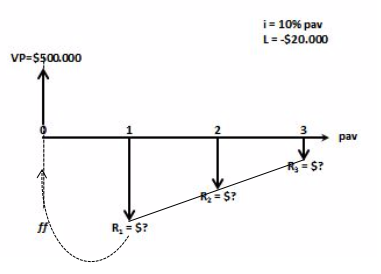
\includegraphics[height=5.0cm]{7_32}
\end{center}
\textbf{b.}	Declaración de variables:\\


	VP=\$ 500.000\\
	i=10 \% pav\\
	n=3 \ \ pav\\
	

\textbf{c.}	Declaración de fórmulas:\\
Gradiente aritmético:\\


	$VP =R \frac{1-(1+i)^{-n}}{i}+\frac{L}{i} [\frac{1-(1+i)^{-n}}{i}-n(1+i)^{-n} ]$\hspace{25pt}\textit{valor presente serie uniforme anticipada}\\

\textbf{d.}	Desarrollo matemático:\\
Procedemos a calcular la primera cuota en pesos de hoy.\\


	$\$ 500.000=R_{1}  \frac{1-(1+i)^{-n}}{i}+\frac{L}{i} [\frac{1-(1+i)^{-n}}{i}-n(1+i)^{-n} ]\\
	\$ 500.000=R_{1} \frac{1-(1+0.10)^{-3}}{0.10}+\frac{(-20.000)}{0.10} [\frac{1-(1+0.10)^{-3}}{0.10}-3(1+0.1)^{-3}]$\\
	


	R = \$219.788,52\\

\textbf{e.}	Respuesta:\\
Y el valor de las cuotas ya corregidas será:\\


	$R_{1} =\$219.788,52 x (1+0,24)^{1} = \$272.537,76\\
	R_{2} =\$199.788,52 x (1 +0,24)^{2}  = \$307.194,83\\ 
	R_{3}=\$179.788,52 x (1 +0,24)^{3}= \$342.789,12$\\



\begin{spacing}{1.1}
    \begin{center}
        \begin{tabular}{|p{1cm}|p{2cm}|p{3cm}|p{2cm}|p{2cm}||p{3cm}|}
        \hline 
        \rowcolor{white!50}
 \textbf{PER\ (1)}  & \textbf{SALDO (2)=(2)-(6)}& \textbf{SALDO AJUSTADO } & \textbf{INTERESES  (4)=(2)*(i)}& \textbf{PAGO\ (5)=\$R-\$L }& \textbf{AMORTIZACIÓN  (2)=(5)-(4)} \\ \hline                                    

            0 & \$500.000,00 & \$620.000,00 & \$0,00 & \$0,00 & \$ 0,00\\ \hline 
            1 & \$409.462,24  &\$507.733,6  & \$62.000,00  & \$272.537,76 & \$ 1210.537,76 \\ \hline
            2 & \$251.311,67  &\$311.626,47  & \$50.773  & \$307.194,83 &\$256.421,51 \\ \hline
            3 & \$0,00 & \$0,00  & \$31.162,65 & \$342.789,12 & \$311.626,47 \\ \hline      
       

 
\end{tabular}
\end{center}
\end{spacing}



\textbf{Ejemplo 13}\\
Resolver el problema anterior, suponiendo que el gradiente es escalonado con pagos semestrales.\\

\textbf{Solución:}\\
\textbf{a.}	Diagrama de flujo de caja:
\begin{center}
	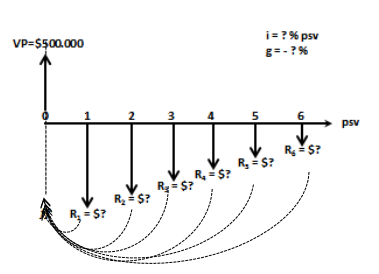
\includegraphics[height=5.0cm]{7_34}
\end{center}
\textbf{b.}	Declaración de variables:\\


	VP=\$ 500.000\\
	i=10 \% \ \ pav\\	
	n=2 \ \ psv\\
	i= ?\%psv\\

\textbf{c.}	Declaración de fórmulas:\\


	$(1 +j)^{m}= (1 +i)^{n} \hspace{35pt} \textit{Equivalencia de tasas}\\
	VF=R \frac{(1+i)^{n}-1}{i}$\hspace{35pt} \textit{valor presente serie uniforme}

\textbf{d.}	Desarrollo matemático:\\
Comenzamos por hallar la tasa de interés periódico semestre vencido.\\


	$(1 +0,1)^{1}= (1 +i)^{2}  \\  i= 4.8808848 \% \ \ psv$\\

Ahora hallaremos la tasa de corrección periódica semestre vencido

	$(1 +0,24)^{1}= (1 +i)^{2}, \ \\ i= 11,3552873 \% \ \ psv$

Si dividimos cada R del ejemplo anterior en dos intercuotas nos queda el valor de cada intercuota en pesos de hoy.\\


	$R_{1}  \frac{(1+0,048808848)^{2}-1)}{0,048808848}= \$ 107.276,24$\\
	
	$R_{3}  \frac{(1+0,048808848)^{2}-1}{0,048808848}=\$ 97.614,48$\\
	
	$R_{5}  \frac{(1+0,048808848)^{2}-1}{0,048808848}=\$ 87.752,71$\\

Y las cuotas ya corregidas quedarán así:\\


	$R_{1}= 107.276,24 x (1 +0,113552873)^{1}= \$119. 457,77$ \\
	
	$R _{2}= 107.276,24 x (1 +0,113552873)^{2}= \$133. 022,54$ \\
	
	$R_{3}=\$97.51,48 x (1 +0,113552873)^{3}= \$134. 648,54$\\
	
	$R_{4}=\$97.514,48 x (1 +0,113552873)^{4}= \$149. 938,26$\\
	
	$R_{5}=\$87.752,71 x (1+0,113552873)^{5}= \$150. 250,09$\\
	
	$R_{6}=\$87.752,71 x (1 +0,113552873)^{6}=\$167. 311,42$\\
	

\textbf{e.}	Respuesta:\\
Y ahora procederemos a elaborar la tabla teniendo en cuenta que la tasa para ajustar el saldo será 11,3552873\% y la tasa para calcular los intereses será el 4,8808848\%


\begin{spacing}{1.1}
    \begin{center}
        \begin{tabular}{|p{1cm}|p{2cm}|p{3cm}|p{2cm}|p{2cm}||p{3cm}|}
        \hline 
        \rowcolor{white!50}
 \textbf{PER\ (1)}  & \textbf{SALDO (2)=(2)-(6)}& \textbf{SALDO AJUSTADO } & \textbf{INTERESES  (4)=(2)*(i)}& \textbf{PAGO\ (5)=\$R-\$L }& \textbf{AMORTIZACIÓN  (2)=(5)-(4)} \\ \hline                                    

            0 & \$500.000,00 & \$556.776,44 & \$0,00 & \$0,00 & \$ 0,00\\ \hline 
            1 & \$464.494,29  &\$517.238,95  & \$27.175,62  & \$119.457,77 & \$ 92.282,15 \\ \hline
            2 & \$409.562,25  &\$455.957,86  & \$25.245,84  & \$133.022,54 &\$107.776,70 \\ \hline
            3 & \$343.564,10 & \$382.576,79 & \$ 22.245,84 & \$134.648,54  & 112.393,76\\ \hline 
            4 & \$251.311,66 & \$279.848,82 &  \$18.673,13 & \$149.938,26 & 131.265,13 \\ \hline 
            5 & \$143.257,83 & \$159.525,17 &  \$13.659,10 & \$150.250,09 & 136.590,99\\ \hline 
            6 & \$0,00 & \$0,00 & \$7.786,24 & \$167.311,41 & \$159.424,17 \\ \hline 
       

 
\end{tabular}
\end{center}
\end{spacing}
\textbf{Ejemplo 14}\\
Elaborar una tabla para amortizar una deuda de US\$10.000 en 3 pagos anuales efectuados en pesos, con una tasa del 18\% periódico anual vencido. Suponga que el tipo de cambio actual es US\$1 = \$900 y que la tasa de devaluación del peso frente al dólar es para el primer año del 15\%, del 27\% para el segundo año y del 13\% para el tercer año.\\

\textbf{Solución:}
\textbf{a.}	Diagrama de flujo de caja:
\begin{center}
	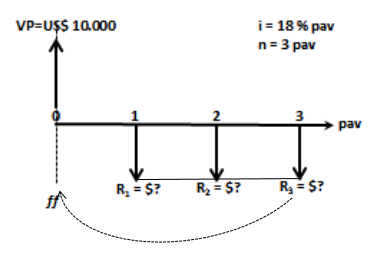
\includegraphics[height=5.0cm]{7_36}
\end{center}
\textbf{b.	}Declaración de variables:\\


	VP=\$ 10.000\\
	i= 18 \% \ \ pav\\
	n=3 \ \ pav\\
	

\textbf{c.}	Declaración de fórmulas:\\


	$VP=R \frac{1-(1+i)^{-n}}{i}$\\\hspace{35pt} \textit{valor presente} 

\textbf{d.}	Desarrollo matemático:\\
Primero calculamos las cuotas en dólares así:\\


	$\$10.000=\frac{R 1-(1+0.18)^{-3}}{0.18}$ \hspace{35pt} \textit{Ecuación de valor}\\
	
	R=US \$ 4.599,24\\
	

Cada año habrá que pagar US \$ 4.599,24, pero como la deuda se va a cancelar en pesos entonces cada año habrá que pagar más pesos por los mismos dólares, por tanto el valor en pesos de cada cuota será:\\


	$R_{1}  = US\$4.599,24 x 900(1 +0,15)=\$4'760.213 \\
	R_{2}  = US\$4'599,24 x 900(1 +0,15)(1+0,27)=\$6'045.471 \\
	R_{3}  = US\$4'599,24 x 900(1 +0,15)(1+0,27)(1+0,13)=\$6.831,382$\\

En el período 0, el saldo se ajusta con la tasa de devaluación del 15\% y así se obtiene el saldo ajustado en cero \$ 9'000.000 x (1 +0,15) = \$ 10'350.000.\\

Sobre este último capital se calculan los intereses al 18\%
\begin{align*}
	\$ 10'350.000 x 0,18=\$ 1'863.000
\end{align*}
La amortización será: cuota – intereses:
\begin{align*}
	\$ 4'760.213 -\$1'863.000 =  \$2'897.213
\end{align*}
El nuevo saldo será: saldo ajustado anterior – amortización:
\begin{align*}
	\$ 10'350.000-\$ 2'897.213 =\$ 7'452.787 
\end{align*}
Este último saldo se ajusta con el 27\% así: 
\begin{align*}
	\$7'452.787 x (1 +0,27) = \$9'465.039
\end{align*}
\textbf{e.}	Respuesta:\\
Los intereses:	$\$ 9'465.039 x 0,18=\$ 1' 703.707$\\
Amortización: 	$\$ 6'045.471 -\$ 1'703.707=\$ 4'341. 764$
Saldo: 		$\$ 9'465.039 -\$ 4'341.764=\$ 5'123.275$		
Saldo ajustado:	$\$ 5'123.275 x (1 + 0,13)=\$ 5'789.301$



\begin{spacing}{1.1}
    \begin{center}
        \begin{tabular}{|p{1cm}|p{2cm}|p{2.5cm}|p{3cm}|p{2cm}||p{3cm}|}
        \hline 
        \rowcolor{white!50}
 \textbf{PER\ (1)}  & \textbf{SALDO (2)=(2)-(6)}& \textbf{SALDO AJUSTADO } & \textbf{INTERESES  (4)=(2)*(i)}& \textbf{PAGO\ (5)=\$R-\$L }& \textbf{AMORTIZACIÓN  (2)=(5)-(4)} \\ \hline                                    

            0 & \$9'000.000,00 & \$10'350.000,00 & \$0,00 & \$0,00 & \$ 0,00\\ \hline 
            1 & \$7'452.787,00  &\$9'465.039,00  & \$1'863.000,00  & \$4'760.213,00 & \$ 2'897.213,00 \\ \hline
            2 & \$5'123.275,00  &\$5'789.301,00  & \$1'703.707,00  & \$6'045.471,00 &\$4'341.764,00 \\ \hline
            3 & \$6,00 & \$6,00 & \$ 1'042.074,00 & \$6'831.382,00  & \$ 5'789.307,00\\ \hline 
             
\end{tabular}
\end{center}
\end{spacing}
\
La diferencia en el resultado final se debe a errores de aproximación en el cálculo de las cuotas, en la liquidación de intereses y en el cálculo del saldo ajustado.\\

\textbf{Ejemplo 15}\\
Una deuda de \$30 millones a una tasa del 6\% periódica, se va a cancelar mediante 5 pagos en la siguiente forma: (el porcentaje de abono a la deuda ha sido pactado inicial- mente entre deudor y acreedor).\\

\textbf{Solución:}
%\begin{center}
%	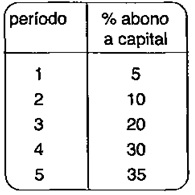
\includegraphics[height=3.5cm]{7_38}
%\end{center}
 
 \begin{spacing}{1.1}
    \begin{center}
        \begin{tabular}{|p{1.5cm}|p{2cm}|}
        \hline 
        \rowcolor{white!50}
            \textbf{FECHA} & \textbf{ABONO A CAPITAL}  \\ \hline                        

           
            1 & \ 5\% \\ \hline
            2 & \ 10\% \\ \hline
            3 & \ 20\% \\ \hline
            4 &\ 30\% \\ \hline
            5 & \ 35\% \\ \hline
            
\end{tabular}
\end{center}
\end{spacing}

\begin{center}
	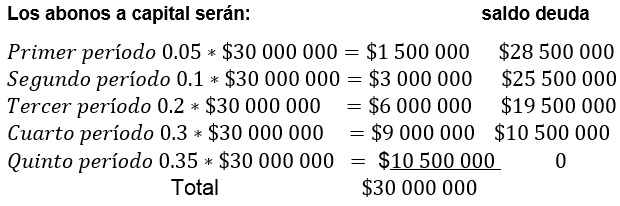
\includegraphics[height=3.5cm]{7_39}
\end{center}
Los intereses se liquidan vencidos sobre el saldo de la deuda, por tanto los intereses serán:\\

En el segundo período $\$28'500.000 x 0,06 = \$1'548. 000$\\
En el tercer período $\$25'500.000 x 0,06= \$1'530.000$ y así sucesivamente.\\

El pago de cada período se obtiene sumando los intereses con la amortización, así para el primer período será: \$1'800.000 + \$1'500.000 = \$3'300.000\\

La tabla total es la siguiente:
%\begin{center}
%	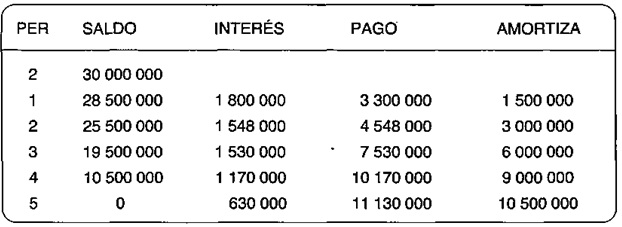
\includegraphics[height=3.5cm]{7_40}
%\end{center}

\begin{spacing}{1.1}
    \begin{center}
        \begin{tabular}{|p{1.5cm}|p{2.5cm}|p{2.3cm}|p{2cm}|p{3.5cm}|}
        \hline 
        \rowcolor{white!50}
            \textbf{PER} & \textbf{SALDO (2)=P-(5)} & \textbf{INTERESES  (3)=P*(i)}& \textbf{PAGO\ (4)}& \textbf{AMORTIZACÍON  (5)=(4)-(3)} \\ \hline                        

           
            2 & \$30´000.000,00  &\$ -------- & \$ ---------  & \$-------  \\ \hline
            1 & \$28'500.000,00  &\$1'800.000,00 & \$3'300.000,00  & \$1'500.000,00\\ \hline
            2 & \$25'500.000,00  &\$1'548.000,00  & \$4'548.000,00  & \$3'000.000,00\\ \hline
           3 & \$ 19'500.000,00 &\$1'530.000,00 & \$7'530.000,00  & \$6'000.000,00 \\ \hline
           4 & \$10'000.000,00  &\$ 1'170.000,00& \$10'170.000,00  & \$9'000.000,00 \\ \hline
            5 & \$0  &\$630.000,00 & \$11'130.000,00   & \$10'500.000,00 \\ \hline
\end{tabular}
\end{center}
\end{spacing}

\textbf{Ejemplo 16}\\
Supongamos que el día 15 de septiembre de 2001 se concede un préstamo por \$5 millones a la tasa DTF + 15 puntos, pagadero en cuotas periódicas trimestrales vencidas a un plazo de 15 meses. Elaborar la tabla de amortización:\\

\textbf{Solución}\\
\textbf{a.}	Diagrama de flujo de caja:
\begin{center}
	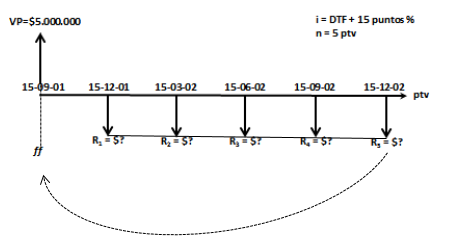
\includegraphics[height=5.0cm]{7_41}
\end{center}
\textbf{b.}	Declaración de variables:
\begin{align*}
	VP=\$ 5.000.000
\end{align*}
\textbf{c.}	Declaración de fórmulas:
\begin{align*}
	VP=R \frac{1-(1+i)^{-n}}{i}\hspace{35pt}\textit{Valor presente}
\end{align*}
\textbf{d.}	Desarrollo matemático:\\
Primero debemos establecer la tasa con la cual calculamos la cuota fija. El día 15-09-2001, fecha en la cual se concede el crédito, la DTF vigente era del 13.776 \% PTA, entonces la tasa del crédito será: 13.776 + 15 = 28.776\% PTA. \\

Como las cuotas son trimestrales debemos usar la tasa periódica trimestral. $\frac{28.776}{ 4} = 7.194\% NTV.$\\

La gráfica nos muestra el plan de amortización. La $R$ representa la cuota fija y la X es el pago final que debe hacerse conjuntamente con la última cuota fija. \\

Cálculo de la cuota fija:
\begin{align*}
	VP=R \frac{1-(1+i)^{-n}}{i}
\end{align*}
\begin{align*}
	\$ 5'000.000 = R \frac{1-(1+0,07194)^{-5}}{0,07194}\ \  de \\
	 R = \$ 1'225.794,51\\
	 
\end{align*}
Los intereses se calculan con la tasa DTF NTA vigente en la fecha en que se debe pagar la cuota, por tanto, no se puede elaborar la tabla total desde un principio, sino en la medida en que se va llegando a la fecha de pago de la cuota, la tabla completa solo se podrá tener el 12-12-02.\\

Aquí daremos las tasas vigentes en cada fecha.
%\begin{center}
%	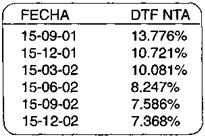
\includegraphics[height=3.5cm]{7_42}
%\end{center}
\begin{spacing}{1.1}
    \begin{center}
        \begin{tabular}{|p{1.5cm}|p{2.5cm}|}
        \hline 
        \rowcolor{white!50}
            \textbf{FECHA} & \textbf{DTF NTA}  \\ \hline                        

           
            15-09-01 & \ 13.776\% \\ \hline
            15-12-01 & \ 10.721\% \\ \hline
            15-03-02 & \ 10.081\% \\ \hline
            15-06-02 &\ 8.247\% \\ \hline
            15-09-02 & \ 7.586\% \\ \hline
            15-12-02 & \ 7.368\% \\ \hline
\end{tabular}
\end{center}
\end{spacing}

DTF	 $(15-12-01)= 10,721\% + 15= 25,721\% nata = 6,430\%$ 	efectiva trimestral\\
DTF	 $(15-03-02)= 10,081\% + 15= 25,081\% nata = 6,270\%$ 	efectiva trimestral\\
DTF	 $(15-06-02)= 8,247\% + 15= 23,247\% nata = 5,812\% $	efectiva trimestral\\
DTF	 $(15-19-02)= 7,586\% + 15= 22,586\% nata = 5,647\% $	efectiva trimestral\\
DTF	 $(15-12-02)= 7,368\% + 15= 25,368\% nata = 5,52\%$ 	efectiva trimestral\\

\textbf{e.}	Respuesta:\\
La amortización del 15-12-02 (\$974.453,95) debe ser igual a la deuda el 15-09-02.
La forma de calcular el pago del 15-12-02 (\$1'028.945,41) debe ser igual a la suma de la amortización con el interés, esto es: 974.453,95 +54.491,46 = 1'028.945,41 La tabla queda así:


\begin{spacing}{1.1}
    \begin{center}
        \begin{tabular}{|p{1.5cm}|p{2.5cm}|p{2cm}|p{2cm}|p{3.5cm}|p{1.5cm}|}
        \hline 
        \rowcolor{white!50}
            \textbf{FECHA} & \textbf{SALDO (2)=P-(5)} & \textbf{INTERESES  (3)=P*(i)}& \textbf{PAGO\ (4)}& \textbf{AMORTIZACÍON  (5)=(4)-(3)}& \textbf{TASA} \\ \hline                        

           
            15-09-01 & \$5´000.000,00  &\$ -------- & \$ ---------  & \$------- &\  ------- \\ \hline
            15-12-01 & \$4'095.705,49  &\$321.500,00 & \$1'225.794,51  & \$904.294,51 &\ 6.430\% \\ \hline
            15-03-02 & \$3'126.711,41  &\$256.800,73  & \$1'225.794,51  & \$968.993,78 &\ 6.270\% \\ \hline
            15-06-02 & \$ 2'082.641,68 &\$181.724,48 & \$1'225.794,51  & \$1'044.070,03&\ 5.812\% \\ \hline
            15-09-02 & \$974.453,95  &\$ 117.606,78& \$1'225.794,51  & \$1'108.187,73 &\ 5.647\% \\ \hline
            15-12-02 & \$0  &\$54.491,95 & \$1'028.945,41   & \$974.453,95 &\ 5.592\% \\ \hline
\end{tabular}
\end{center}
\end{spacing}

%\begin{center}
%	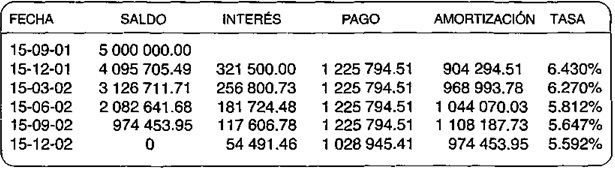
\includegraphics[height=3.5cm]{7_43}
%\end{center}
\textbf{Observación:} En el caso anterior, el deudor salió favorecido porque su última cuota fue inferior a las anteriores, esto se debió a que el cálculo de la cuota fija se hizo con base en una DTF mayor (7.194\% ET), pero, esta tasa vino disminuyendo a lo largo del crédito, si hubiese venido aumentando entonces, el pago del 12-12-02 habría sido mayor. Como consecuencia de lo anterior se deduce que este sistema es más equitativo porque al final se ajusta el pago de acuerdo al comportamiento de las tasas del mercado.\\

\textbf{Ejemplo 17}\\
Para el día 15 de abril de 1998 debe haberse reunido la suma de \$900.000 para tal fin se efectúan depósitos trimestrales de \$R c/u en un fondo que paga el 32\% nominal trimestre vencido. Si el primer depósito se hace el 15 de enero de 1997 y el último el 15 de octubre de 1997:\\

a) Calcular el valor del depósito trimestral\\
b)  Elaborar una tabla de capitalización\\

\textbf{Solución:}
\begin{center}
	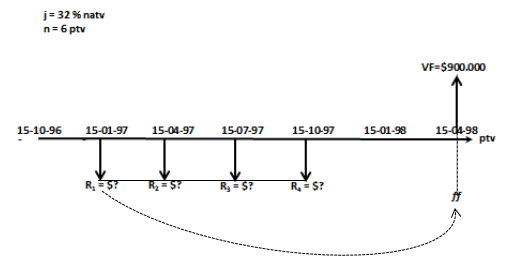
\includegraphics[height=5.0cm]{7_44}
\end{center}
a)	  La ecuación de valor será: 
\begin{align*}
	Rx4(1.08) ^{2}=\$900.000
\end{align*}
 $ R = \$17. 235,19$\\

\textbf{Respuesta: }
b)

\begin{spacing}{1.1}
    \begin{center}
        \begin{tabular}{|p{1cm}|p{2.5cm}|p{2cm}|p{2cm}|p{3.5cm}|}
        \hline 
        \rowcolor{white!50}
            \textbf{PER\ (1)} & \textbf{ACOMULADO (2)=(2)+(5)} & \textbf{INTERESES  (3)=P*(i)}& \textbf{DEPOSITO\ (4)}& \textbf{CAPITALIZACÍON  (5)=(4)+(3)} \\ \hline                        

           
            1 & \$171.235,19  &\$ -------- & \$171.235,19   & \$171.235,19 \\ \hline
            2 & \$356.169,20 &\$ 13.698,82 & \$171.235,19   & \$184.934,01 \\ \hline
            3 & \$555.897,93 & \$28.493,54  & \$171.235,19  & \$199.728,73 \\ \hline
            4 & \$771.604,95  & \$44.471,83 & \$171.235,19   & \$215.707,02 \\ \hline
            5 & \$833.333,35 & \$61.728,40 & \$---------- & \$61.728,40 \\ \hline
            6 & \$900.000,02  & \$66.666,67& \$----------  & \$66.666,67 \\ \hline

 
\end{tabular}
\end{center}
\end{spacing}


Observación: el error de \$0.02 se debe a la aproximación en el valor de la cuota.\\

\textbf{Ejemplo 18}\\
Se desean reunir \$800.000 en 4 depósitos periódicos crecientes en un 20\% más una cuota extra pactada de \$80.000 en el período 2. Con una tasa del 20\% efectiva para el período. Elabore la tabla de capitalización.\\

\textbf{Solución:}\\
\textbf{a.}	Diagrama de flujo de caja:
\begin{center}
	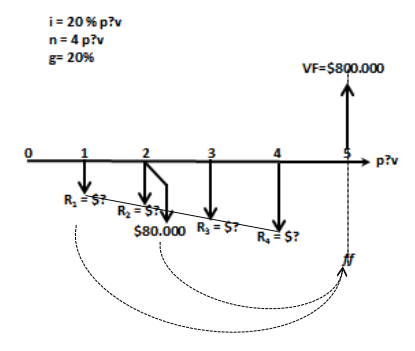
\includegraphics[height=5.0cm]{7_46}
\end{center}
\textbf{b.}	Declaración de variables:\\


	VF=\$800.000\\
	i = 20\%p?v\\
	n=4 p?v\\	
	g=20\%\\
	R=\$80.000\\
	
\textbf{c.}	Declaración de fórmulas:\\


	$VF=R_{n}(1+i)^{n-1}$ \hspace{35pt}\textit\\

\textbf{d.}	Desarrollo matemático:\\
En este caso se trata de un gradiente geométrico en el cual g = i= 20\% por lo tanto la    ecuación de valor será:\\

	$\$800.000 =R_{1}  (4) (1 +0,2)^{3}  + 80.000(1 +0,2)^{2}$\\

	$R_{1}  =\$99.074,07 \\
	R_{2}  =\$99.074,07 (1 +0,2)^{1}=\$118.888,89+80.000=\$198.888,89\\
	R_{3}  =\$99.074,07 (1 +0,2)^{2}=\$142.666,67\\
	R_{4}  =\$99.074,07 (1 +0,2)^{3}=\$171.200,00$

\textbf{e.}	Respuesta:
%\begin{center}
%	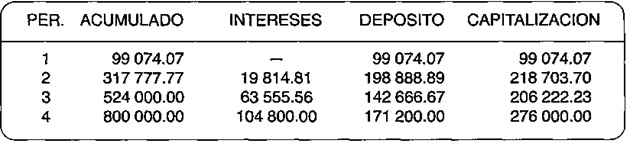
\includegraphics[height=3.5cm]{7_47}
%end{center}

\begin{spacing}{1.1}
    \begin{center}
        \begin{tabular}{|p{1cm}|p{2.5cm}|p{2cm}|p{2cm}|p{3.5cm}|}
        \hline 
        \rowcolor{white!50}
            \textbf{PER\ (1)} & \textbf{ACOMULADO (2)=(2)+(5)} & \textbf{INTERESES  (3)=P*(i)}& \textbf{DEPOSITO\ (4)}& \textbf{CAPITALIZACÍON  (5)=(4)+(3)} \\ \hline                        

           
            1 & \$99.074,07  &\$ -------- & \$99.074,07  & \$99.074,07 \\ \hline
            2 & \$317.777,77 &\$ 19.814,81 & \$198.888,89  & \$218.703,70 \\ \hline
            3 & \$524.000,00 & \$63.555,56  & \$142.666,67 & \$206.222,23 \\ \hline
            4 & \$800.000,00  & \$104.800,00 & \$171.200,00  & \$276.000,00 \\ \hline

 
\end{tabular}
\end{center}
\end{spacing}

\textbf{Ejemplo 19}\\
Supongamos que tenemos que pagar la suma de \$800.000 al final de 2 años y mientras tanto debemos pagar intereses a la tasa del 3\% mensual vencido. Con el fin de ir reuniendo el dinero necesario para cancelar la deuda se constituye un fondo mediante depósitos mensuales iguales que ganan un interés del 2.5\% efectivo mensual. Calcular el costo mensual de la deuda.\\

\textbf{Solución:}\\
\textbf{a.}	Diagrama de flujo de caja:
\begin{center}
	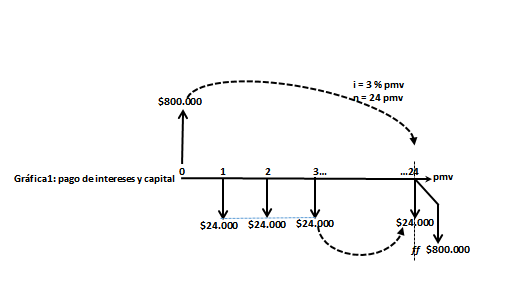
\includegraphics[height=9cm]{7_48}
\end{center}
\begin{center}
	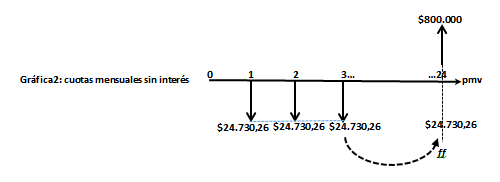
\includegraphics[height=5.5cm]{7_49}
\end{center}
Mensualmente debemos pagar un interés de \$800.000 x 0,03 = \$24.000
Por otra parte, el depósito mensual en el fondo será:
\$800.000 = Rx24 (1,025); \\R =  \$24.730,26
Y el costo mensual de la deuda será: 24.000 + 24.730,26 = \$48.730,26\\

\textbf{b.}	Respuesta:\\
La primera gráfica representa el pago de intereses y la deuda, la segunda gráfica representa los depósitos en el fondo y el capital reunido, al final de los 2 años se cancela el fondo y con ese dinero se paga la deuda.\\

\textbf{Observación:} cuando la capitalización se hace mediante cuotas crecientes, por ejemplo con un gradiente, entonces el costo de la deuda de cada período es variable.\\

\textbf{Ejemplo 20}\\
Se adquiere una propiedad a un costo de seis millones de pesos dando una cuota inicial del 30\% y el saldo será pagadero al final de 3 años, mientras tanto se pagarán intereses por mes anticipado al 3\%. Con el objeto de cancelar la deuda a su vencimiento, se constituye un fondo que paga el 33\% nominal mes vencido mediante depósitos mensuales ordinarios crecientes en \$2.000. Determinar el costo del período 15.\\

\textbf{Solución:}\\
\textbf{a.}	Diagrama de flujo de caja:
\begin{center}
	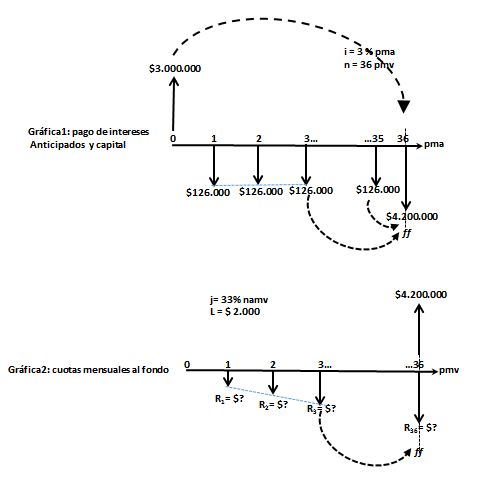
\includegraphics[height=10.0cm]{7_50}
\end{center}
\textbf{b.}	Declaración de variables:
\begin{align*}
	Interes: 	\$4'200.000 x  0,03 = \$126.000
\end{align*}
\textbf{c.}	Declaración de fórmulas:
\begin{align*}
	VF=Rn(1+i)^{n-1}\\
	R_{n}= R_{1}+ (n- 1)L
\end{align*}
\textbf{d.}	Desarrollo matemático:
\begin{align*}
	\$4'200.000 = R_{1} + (36)(2,75\%)+  \frac{2.000}{0,0275}  [(36)(2,75\%)-36]
\end{align*}
\textbf{e.}	Respuesta:\\

	$R_{1}=\$40.531,73$\\

	  
\begin{align*}
	R_{15}=\$40.531,73 + (15 -1)(2.000) = \$68.531,73
\end{align*}
Esto significa que en el período 15 el deudor debe disponer de \$194.531,73 de los cuales \$126.000 los dedica al pago de intereses y el resto (\$68.531,73) se deposita en el fondo.\\

\textbf{Observación:} el costo de la deuda en el período 36 será únicamente el valor de la cuota $R_{36}$ que es igual a \$110.531,73.

